\documentclass[11pt]{article}

% --- Essential Packages ---
\usepackage[utf8]{inputenc}
\usepackage{amsmath, amssymb, geometry, listings, xcolor}
\geometry{margin=1in}
\setlength{\parskip}{0.8em}
\setlength{\parindent}{1.5em}
\usepackage{graphicx}        
\usepackage{booktabs}     
\usepackage{caption}
\usepackage{subcaption}      
\usepackage{hyperref}
\hypersetup{
    colorlinks=true,
    linkcolor=blue,
    filecolor=magenta,      
    urlcolor=cyan,
}
\usepackage{listings}
\usepackage{xcolor}

% Define custom colors for code aesthetics
\definecolor{codegreen}{rgb}{0,0.6,0}
\definecolor{codegray}{rgb}{0.5,0.5,0.5}
\definecolor{codepurple}{rgb}{0.58,0,0.82}
\definecolor{backcolour}{rgb}{0.95,0.95,0.92}

\lstdefinestyle{mystyle}{
    backgroundcolor=\color{backcolour},   
    commentstyle=\color{codegreen},
    keywordstyle=\color{magenta},
    numberstyle=\tiny\color{codegray},
    stringstyle=\color{codepurple},
    basicstyle=\ttfamily\footnotesize,
    breakatwhitespace=false,         
    breaklines=true,                 
    captionpos=b,                    
    keepspaces=true,                 
    numbers=left,                    
    numbersep=5pt,                  
    showspaces=false,                
    showstringspaces=false,
    showtabs=false,                  
    tabsize=2,
    frame=single % Adds a professional box around the code
}

\lstset{style=mystyle}

\usepackage{subcaption}

% --- Document Information ---
\title{CFD Project 1}
\author{Ben Rees}
\date{\today}

\begin{document}

\maketitle

\section{Introduction}
In this project, the parabolic equation with boundary conditions as listed below is solved analytically and via a 
numerical discretization scheme. The results are compared and discussed.

Parabolic Equation:
$$
\frac{\partial u}{\partial x}-2\frac{\partial^2 u}{\partial y^2}=2.
$$

Boundary and Initial Conditions:
$$
u(x,0)=0,\quad u(x,1)=0,\quad u(0,y)=0.
$$

\section{Analytical Solution Derivation}
The governing equation $\frac{\partial u}{\partial x}-2\frac{\partial^2 u}{\partial y^2}=2$ is linear but inhomogeneous. Using the 
principle of superposition, we define $u(x,y) = v(x,y) + f(y)$, where $f(y)$ is the steady-state solution and $v(x,y)$ is the 
transient homogeneous component.

\subsection{Steady-State Solution}
To homogenize the PDE, we require $f(y)$ to satisfy $-2f''(y) = 2$, or $f''(y) = -1$. Applying boundary conditions $f(0)=f(1)=0$:
\begin{align*}
    f(y) &= -\frac{y^2}{2} + C_1 y + C_2 \xrightarrow{BCs} f(y) = \frac{y}{2}(1-y).
\end{align*}

\subsection{Transient Solution via Separation of Variables}
The remaining homogeneous equation $\frac{\partial v}{\partial x} - 2\frac{\partial^2 v}{\partial y^2} = 0$ is solved assuming
 $v(x,y) = X(x)Y(y)$. Separating variables yields:
\begin{equation*}
    \frac{X'}{2X} = \frac{Y''}{Y} = -\lambda^2 \implies 
    \begin{cases} 
    Y'' + \lambda^2 Y = 0, & Y(0)=Y(1)=0 \\
    X' + 2\lambda^2 X = 0
    \end{cases}.
\end{equation*}
Solving the eigenvalue problem gives $\lambda_n = n\pi$ and eigenfunctions $Y_n(y) = \sin(n\pi y)$ for $n=1,2,3..$. The temporal
solution is $X_n(x) = e^{-2(n\pi)^2x}$. By superposition:
\begin{equation*}
    v(x,y) = \sum_{n=1}^\infty B_n \sin(n\pi y) e^{-2(n\pi)^2x}.
\end{equation*}
Using the initial condition $u(0,y)=0 \implies v(0,y) = -f(y)$, the Fourier coefficients $B_n$ are calculated via orthogonality:
\begin{equation*}
    B_n = 2 \int_0^1 -\frac{y}{2}(1-y) \sin(n\pi y) dy = \frac{2}{(n\pi)^3} [(-1)^n - 1].
\end{equation*}
The final analytical solution is $u(x,y) = \frac{y}{2}(1-y) + \sum_{n=1}^\infty B_n \sin(n\pi y) e^{-2(n\pi)^2x}$.

\section{Numerical Discretization and Implementation}
In this report, a finite volume method based on the central difference approximation with a Crank-Nicolson time-stepping scheme 
is employed due to this scheme's second-order accuracy, stability, and conservativeness. The spatial domain (1D) is discretized into
$M$ control volumes with uniform spacing $\Delta y = 1/M$. The temporal domain is discretized with a time step $\Delta x$.
The current time is denoted by $x^N$ and the center gridpoint is denoted by $y_i$:
$$
\int_{x^N}^{x^{N+1}}\int_{V_i}\left(\frac{\partial u}{\partial x}\right)dVdx=\int_{x^N}^{x^{N+1}}\int_{V_i}
2\frac{\partial^2 u}{\partial y^2}dVdx+\int_{x^N}^{x^{N+1}}\int_{V_i}2dVdx.
$$
This becomes:
$$
(u^{N+1}_i-u^N_i)\Delta y=2\left(\frac{u^{N+1}_{i+1}-2u^{N+1}_i+u^{N+1}_{i-1}}{2(\Delta y)^2}+
\frac{u^{N}_{i+1}-2u^{N}_i+u^{N}_{i-1}}{2(\Delta y)^2}\right)\Delta y\Delta x+2\Delta y\Delta x;
$$
$$
\implies \frac{u^{N+1}_i-u^N_i}{\Delta x}=\frac{1}{(\Delta y)^2}(u^{N+1}_{i+1}-2u^{N+1}_i+u^{N+1}_{i-1}+u^{N}_{i+1}-2u^{N}_i+
u^{N}_{i-1})+2.
$$
Rearranging to fit the linear system form $Au^{N+1}=b$, defining $r=\frac{\Delta x}{(\Delta y)^2}$:
$$
-r u^{N+1}_{i-1}+(1+2r)u^{N+1}_i-r u^{N+1}_{i+1} = r u^{N}_{i-1}+(1-2r)u^{N}_i+r u^{N}_{i+1}+2\Delta x.
$$
This gives the tridiagonal elements of the A matrix for grid points in the center. Applying the boundary conditions with the 
half-cell approach to maintain cell-centered FVM consistency, the first and last rows of the A matrix instead use the form:
$$
(1+6r)u_1^{N+1}-2ru_2^{N+1}=(1-6r)u_1^{N}+2ru_2^N+2\Delta x\quad\text{(Left BC), and}
$$
$$
-2ru_{M-1}^{N+1}+(1+6r)u_M^{N+1}=2ru_{M-1}^{N}+(1-6r)u_M^{N}+2\Delta x\quad\text{(Right BC).}
$$
The general flow of the numerical implementation is as follows:
\begin{enumerate}
    \item Initialize parameters: $M$, $Nt$ (number of time steps), $\Delta y$, $\Delta x$, and the solution array $u$ with initial
     conditions.
    \item Construct the A matrix based on the discretization scheme and boundary conditions.
    \item For each time step, compute the right-hand side vector $b$, then solve for $u^{N+1}$ using 
    \lstinline|scipy.linalg.solve_banded| (TDMA).
    \item Make the previous solution $u^{N+1}$ the current solution $u^N$ and repeat the previous step until the desired
     final time is reached.
\end{enumerate}
The implementation is done in Python, utilizing NumPy for array operations and SciPy for solving the linear system efficiently. 
The TDMA solver is an LU decomposition modification chosen for its suitability to the tridiagonal structure of the A matrix, 
ensuring computational efficiency and stability.
\section{Presentation of Results}
A 3D surface plot of the numerical solution $u(x,y)$ is shown below in Figure \ref{fig:3d_evolution} to illustrate the evolution
 of the solution over time and space. The plot demonstrates the expected behavior of the solution, with the transient component 
 decaying over time and the steady-state solution dominating as $x$ increases. The system behavior closely resemebles the progression
 of a velocity profile in a lamniar channel or pipe.
\begin{figure}[h]
    \centering
    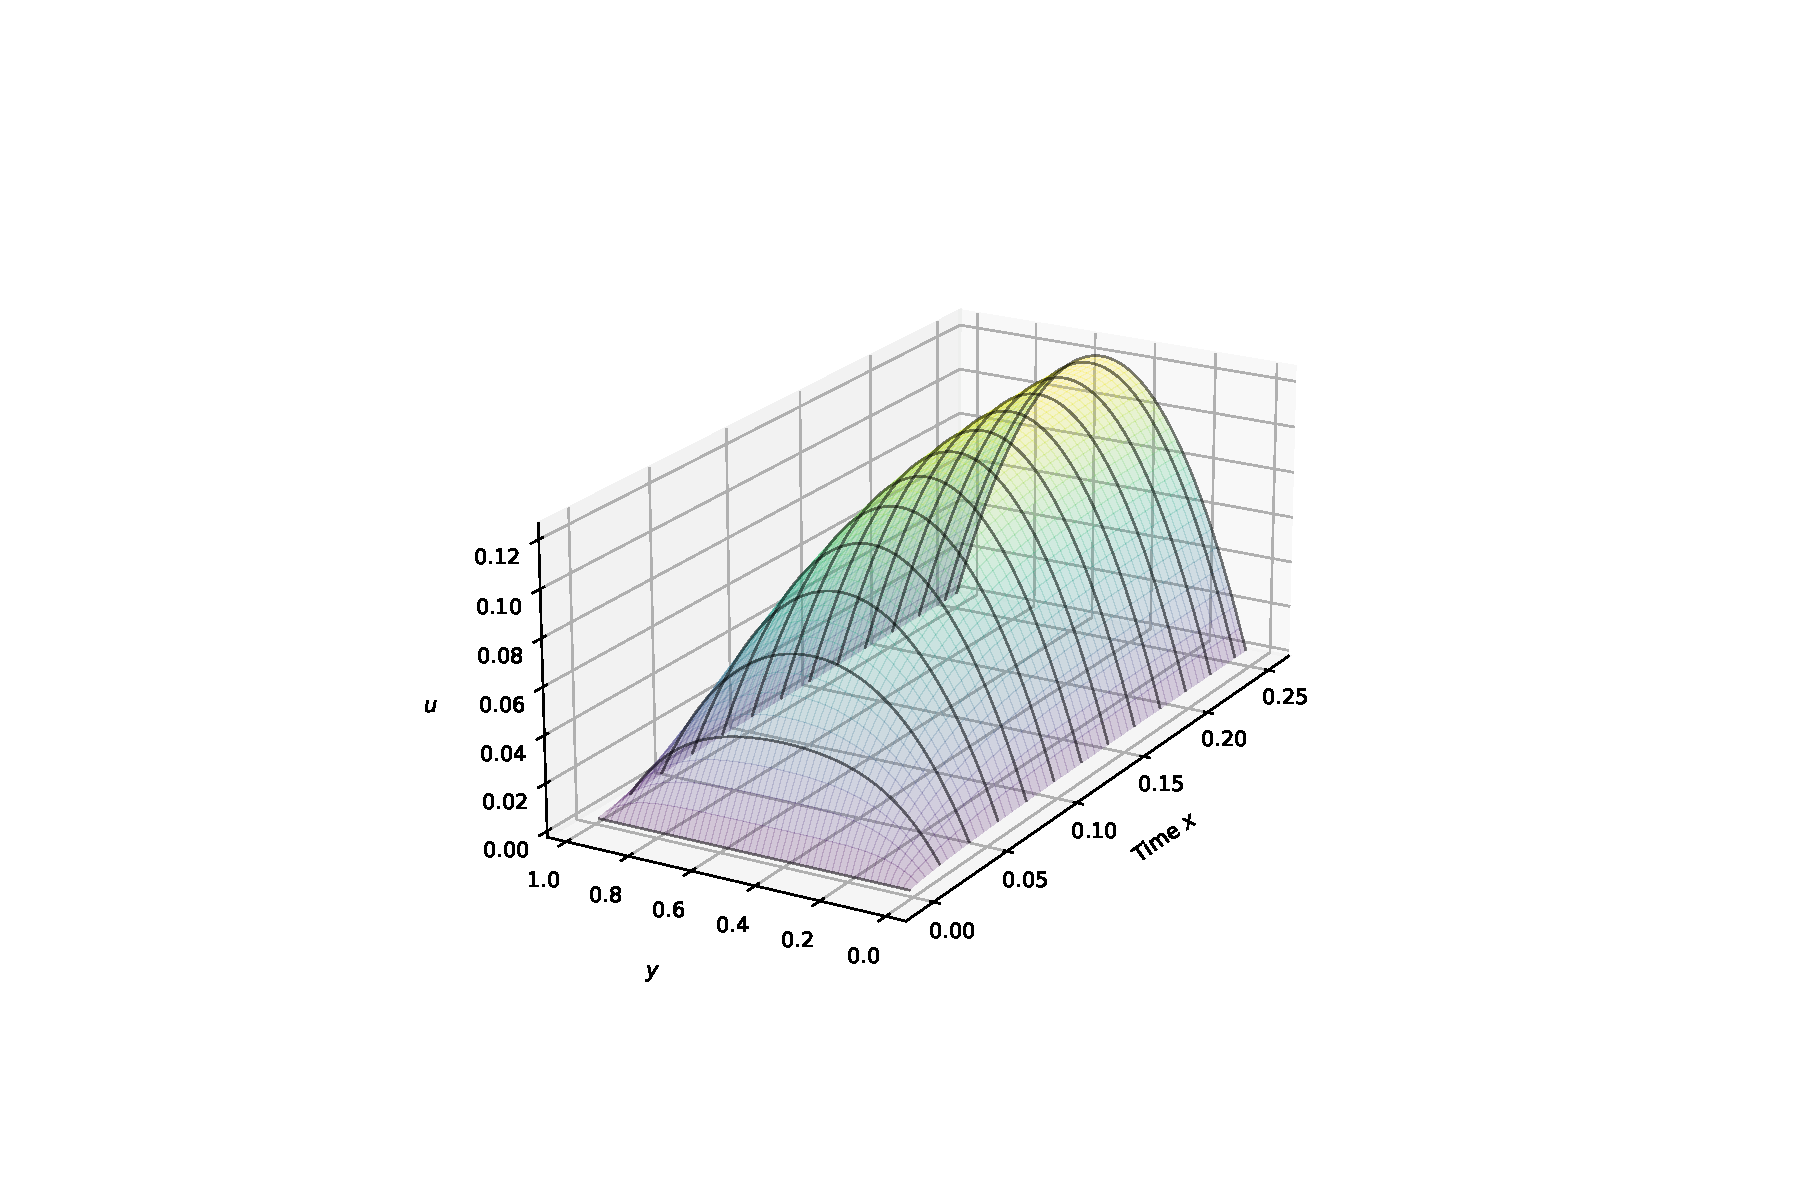
\includegraphics[width=0.8\textwidth]{Figures/iso_dx_0.001.pdf}
    \caption{3D Velocity Profile Development.}
    \label{fig:3d_evolution}
\end{figure}
Comparison of the numerical solution to the analytical solution at various time steps is shown in Figure \ref{fig:comparison}.
 The numerical solution closely matches the analytical solution, with discrepancies decreasing as the time step is reduced,
  demonstrating the convergence of the method.
\begin{figure}[htbp]
    \centering
    \begin{subfigure}[b]{0.8\textwidth}
        \centering
        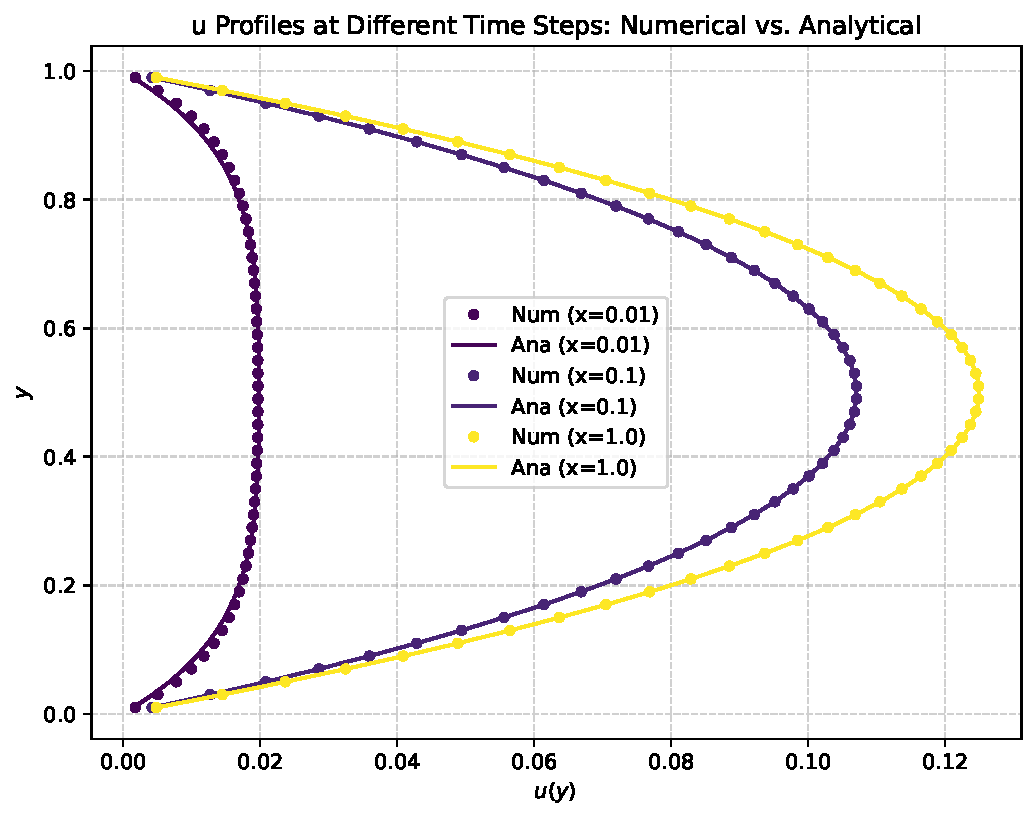
\includegraphics[width=0.8\textwidth]{Figures/u_comparison_dx_0.01.pdf}
        \caption{Large time step ($\Delta x = 0.01$).}
    \end{subfigure}
    \vspace{5mm}
    \\ % This forced line break stacks them
    \begin{subfigure}[b]{0.8\textwidth}
        \centering
        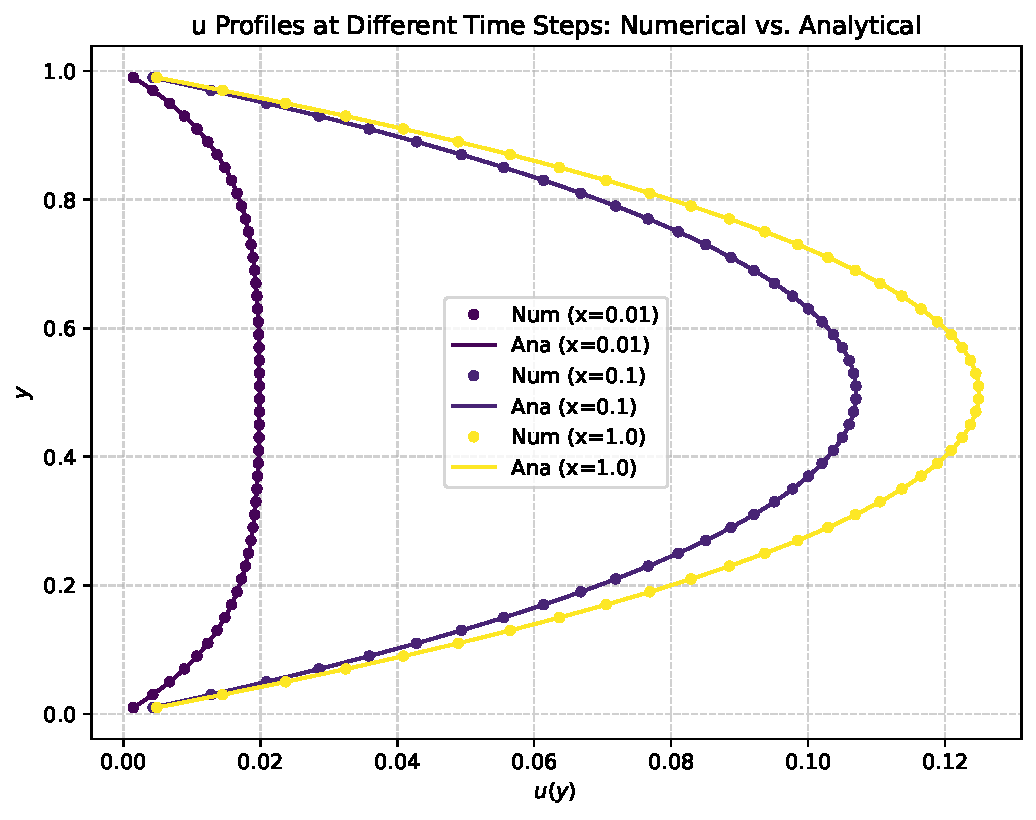
\includegraphics[width=0.8\textwidth]{Figures/u_comparison_dx_0.001.pdf}
        \caption{Small time step ($\Delta x = 0.001$).}
    \end{subfigure}
    \caption{Temporal resolution study.}
    \label{fig:comparison}
\end{figure}

\section{Discussion}
The numerical solution correctly obtains the asymptotic behavior of the solution, and the stability of this scheme and chosen
 grid resolution is demonstrated by:
\begin{enumerate}
    \item The lack of oscillations in the solution sometimes observed in second order schemes even at varying time steps.
    \item Preservation of the boundary conditions throughout the simulation.
    \item Symmetry about the centerline $y=0.5$ is maintained, consistent with the problem's symmetry.
    \item The convergence of the numerical solution to the analytical solution as the time step is reduced, indicating that the 
    method is consistent and stable.
\end{enumerate}

\section{Appendix: Code Listings}
\subsection{physics.py}
\lstinputlisting[language=Python, caption={Physics module containing the analytical solution and coefficients.}]{Modules/physics.py}

\subsection{solvers.py}
\lstinputlisting[language=Python, caption={Numerical solver implementation using the Crank-Nicolson scheme.}]{Modules/solvers.py}

\subsection{post.py}
\lstinputlisting[language=Python, caption={Post-processing and visualization tools.}]{Modules/post.py}

\subsection{main.py}
\lstinputlisting[language=Python, caption={Main script to run the simulation and generate results.}]{Modules/main.py}

\section{Code Availability}
All Python scripts are available on GitHub at: \url{https://github.com/Ben-JaminRees/Fuel-Cell-Course-Spring-2026/tree/main/Assignment_2_2}.

\end{document}